\documentclass[sigconf, nonacm]{acmart}

\usepackage{tabularx}
\newcolumntype{C}{>{\centering\arraybackslash}X} 

\AtBeginDocument{
  \providecommand\BibTeX{{
    Bib\TeX}}}

\acmConference[LEAK '25]{Unusual Side Channels and Privacy Leaks}{Februrary 07, 2025}{Berlin, Germany}
\setcopyright{cc}
\setcctype[4.0]{by-sa}
\acmDOI{}
\acmISBN{}

\begin{document}

\title{Eavesdropping Speech with Non-sensing Devices}

\author{Tim Holzhey}
\affiliation{%
  \institution{Technische Universität Berlin}
  \city{Berlin}
  \country{Germany}}
\email{holzhey@campus.tu-berlin.de}

\begin{abstract}
  % Topic + Relevance
  In recent years, numerous research papers have shown that air pressure waves produced by human speech or other sounds can induce vibrations into an array of non-acoustic sensors (e.g. motions sensors) or into externally measured objects (e.g. laser-based vibrometer) skewing sensor readings in a reversable manner, effectively turning them into undisclosed microphones.
  This allows for eavesdropping on private speech by maliciously altered devices and therefore posing a real threat to privacy when exploited.
  
  % Objective of this paper
  This work will examine and compare different types of vibration-based side channel attacks employed on common IoT and Smart devices to recover speech or infer privacy-sensitive information about the speaker like their identity, political views or gender.
  We explore the steps taken to take control of the targeted device, gather the necessary data, and perform signal processing and machine learning techniques to extract audible information from the sensor readings.
  The overview established over the attacks then allows for a comprehensive feasability study for the respective attack methods and complexity required to perform such attacks in a real world scenario. 
  We discuss possible countermeasures to mitigate the risk of such attacks and provide an outlook on future research directions in the field.
\end{abstract}

\begin{CCSXML}
  <ccs2012>
  <concept>
  <concept_id>10002978.10003001.10010777.10011702</concept_id>
  <concept_desc>Security and privacy~Side-channel analysis and countermeasures</concept_desc>
  <concept_significance>500</concept_significance>
  </concept>
  <concept>
  <concept_id>10002978.10003001.10003003</concept_id>
  <concept_desc>Security and privacy~Embedded systems security</concept_desc>
  <concept_significance>500</concept_significance>
  </concept>
  <concept>
  <concept_id>10010520.10010553.10010559</concept_id>
  <concept_desc>Computer systems organization~Sensors and actuators</concept_desc>
  <concept_significance>500</concept_significance>
  </concept>
  </ccs2012>
\end{CCSXML}

\ccsdesc[500]{Security and privacy~Side-channel analysis and countermeasures}
\ccsdesc[500]{Security and privacy~Embedded systems security}
\ccsdesc[500]{Computer systems organization~Sensors and actuators}

\keywords{Security, Privacy, Side-channel, Eavesdropping, Speech, Acoustic, Hardware Security, Privacy Leaks}

% \begin{teaserfigure}
%   \includegraphics[width=\textwidth]{sampleteaser}
%   \caption{Seattle Mariners at Spring Training, 2010.}
%   \Description{Enjoying the baseball game from the third-base
%   seats. Ichiro Suzuki preparing to bat.}
%   \label{fig:teaser}
% \end{teaserfigure}

\received{7 January 2025}
% \received[revised]{12 March 2009}
% \received[accepted]{5 June 2009}

\maketitle

\section{Introduction}
While the IoT market is on the rise and still growing exponentially, projected to exceed USD 4 trillion by 2032 \cite{FortuneBusinessInsights2024}, this opens up a new attack vector for adversaries to exploit in addition to traditional software vulnerabilities in computers.
Latest surveys show that the American households had on average 21 connected devices \cite{DeloitteConnectedConsumer2023}, a relevant part of which are IoT and Smart Home devices.
IoT devices are often equipped with a variety of sensors to interface with their physical environment, such as accelerometers, gyroscopes, microphones, and cameras.
Many of these sensors can also be found in modern smartphones, which are carried around by most people\footnote{Surveys from 2024 suggest that 91 \% of Americans own a smartphone \cite{PewResearchMobileFactSheet2024}}. Mobile operating systems provide zero-permission access to sensor data from the built-in accelerometer and gyroscope, therefore have been the subject of the majority of research done in this field.
The findings from vulnerabilities found in smartphones can be projected onto IoT and Smart devices with similar sensors that do not have a primary function of audio recording i.e. do not have a built-in microphone ("non-sensing").
To execute a vibration-based eavesdropping attack, most of the previous papers took the approuch to exploited MEMS\footnote{Abbr. Micro-electromechanical systems} motion sensors (accelerometers, gyroscopes and magnetometers) commonly found in smartphones and many smart devices including smartwatches, fitness trackers, gaming controllers, etc.
Some of the more experimental approaches have also shown that other sensors like Lidar scanners in vacuum cleaners, the position error signal of write heads in hard drives or electro-optical sensors directed at ceiling lights can be exploited for similar attacks.

\textbf{CONTRIBUTION:} Altough parts of the available research material in this field is investigating keystroke recovery attacks \cite{Touchtone2023}\cite{TouchLogger2011}\cite{TapLogger2012} or is using sophisticated external setups (e.g. RFID-Tags \cite{RFMic2023}, millimeter-waves \cite{MMMic2022}, WiFi radio \cite{ART2015}), we limit the scope of this paper to \textbf{on-device vibration-based speech and general sound recovery attacks}.
This includes attacks in theory possible without any modified or additional hardware assuming a compromised device or malicious software.
This work aims to provide a comprehensive overview of the current state of research in the field of vibration-based eavesdropping attacks on non-sensing devices.
We highlight notable research papers and their findings, compare the different attack methods and achieved results, and discuss the feasibility of such attacks in real-world scenarios.

\section{Background and Related Work}
\subsection{Vibration-based Eavesdropping Attacks}
Sound created by a human speaking or any other sound can be characterized as spatially and temporally propagating changes in air pressure in the audible frequency range (20 Hz - 20 kHz).
Similarly to how sound waves induce vibrations into our eardrums to let us perceive sound, they can also couple vibrations into all other objects they encounter, more so into objects that are resonant at the frequency of the sound.
In a typical microphone, an oscillating diaphragm is used to convert these vibrations into an electrical signal i.e. a change in voltage by varying the capacitance of a capacitor (condenser microphone) or by inducing a current into a coil (dynamic microphone).
Even if unintended, the same phenomenon can be used to turn any other sensing electrical component into a microphone if it has a moving part capable of influencing the electrical properties of the component directly (e.g. MEMS, write head of a hard drive) or observing the movement of another object (e.g. laser vibrometer, Lidar scanner, camera).
As audible information was not intended to be captured by these sensors, an attacker who is able to recover this information from the sensor readings is exploiting a side channel vulnerability.

\subsection{MEMS-based Eavesdropping Attacks}

Sensors manufactured using micro-electromechanical fabrication techniques (MEMS) incorporate electronics and moving parts on a micrometer-scale chip to measure physical parameters like acceleration (accelerometer), orientation and angular velocity (gyroscope) or the magnetic field (magnetometer).
The manufactureing process makes use of lithography and etching semiconductor manufacturing techniques on silicon wafers that allows for the production of small, low-cost sensors with high sensitivity and accuracy.
They are widely used in consumer electronics to enable features like screen rotation, step counting, navigation and gaming feedback.
On a physical level, MEMS sensors are most commonly realized by a spring-suspended proof mass that changes the capacitance of the circuitry when displaced (variable capacitance MEMS) or by a flexible piezoelectric material that changes its electrical resistance when bent (piezoresistive MEMS).
The structures can be repeated and aligned in three orthogonal directions to measure the physical property in the three-dimensional spacial domain.
\\~\\
\textbf{MEMS Accelerometer:} An accelerometer measures the proper acceleration (change in velocity) of an object relative to a local inertial reference frame.
In the gravitational field of the earth, the accelerometer's measurement is offset by the upwards acceleration of 1 g (9.81 m/s\textsuperscript{2}) relative to the free-falling reference frame.
The basic mechanical structure of an accelerometer consists of a damped proof mass suspended by springs that is displaced when the sensor is accelerated in the opposite direction of movement.
In a typical VC MEMS accelerometer, the proof mass moves between air-gapped fixed electrodes forming a variable capacitor as shown in Figure \ref{fig:MEMS_accelerometer}.
\\[6pt]
\textbf{MEMS Gyroscope:} A gyroscope measures the angular velocity (rate of rotation) of an object relative to a local inertial reference frame.
Gyroscopes realized as a MEMS sensor are commonly Vibrating structure gyroscopes (VSG) that measure the Coriolis force acting on a vibrating proof mass when the sensor is rotated.
As the vibrating mass tends to continue vibrating in the same plane, the Coriolis force deflects the mass in the direction perpendicular to the rotation axis.
The deflection is measured by capacitive sensing or piezoresistive sensing and is proportional to the angular velocity of the rotation as shown in Figure \ref{fig:MEMS_gyroscope}.
\\[6pt]
\textbf{MEMS Magnetometer:} A magnetometer measures the strength and direction of the local magnetic field.
MEMS-based magnetometers often use the Lorentz force acting on the current-carrying conductor in the magnetic field to move the mechanical structure.
The displacement is then measured by capacitive, piezoresistive or optical sensing and is proportional to the magnetic field strength.

\begin{figure}[H]
  \centering
  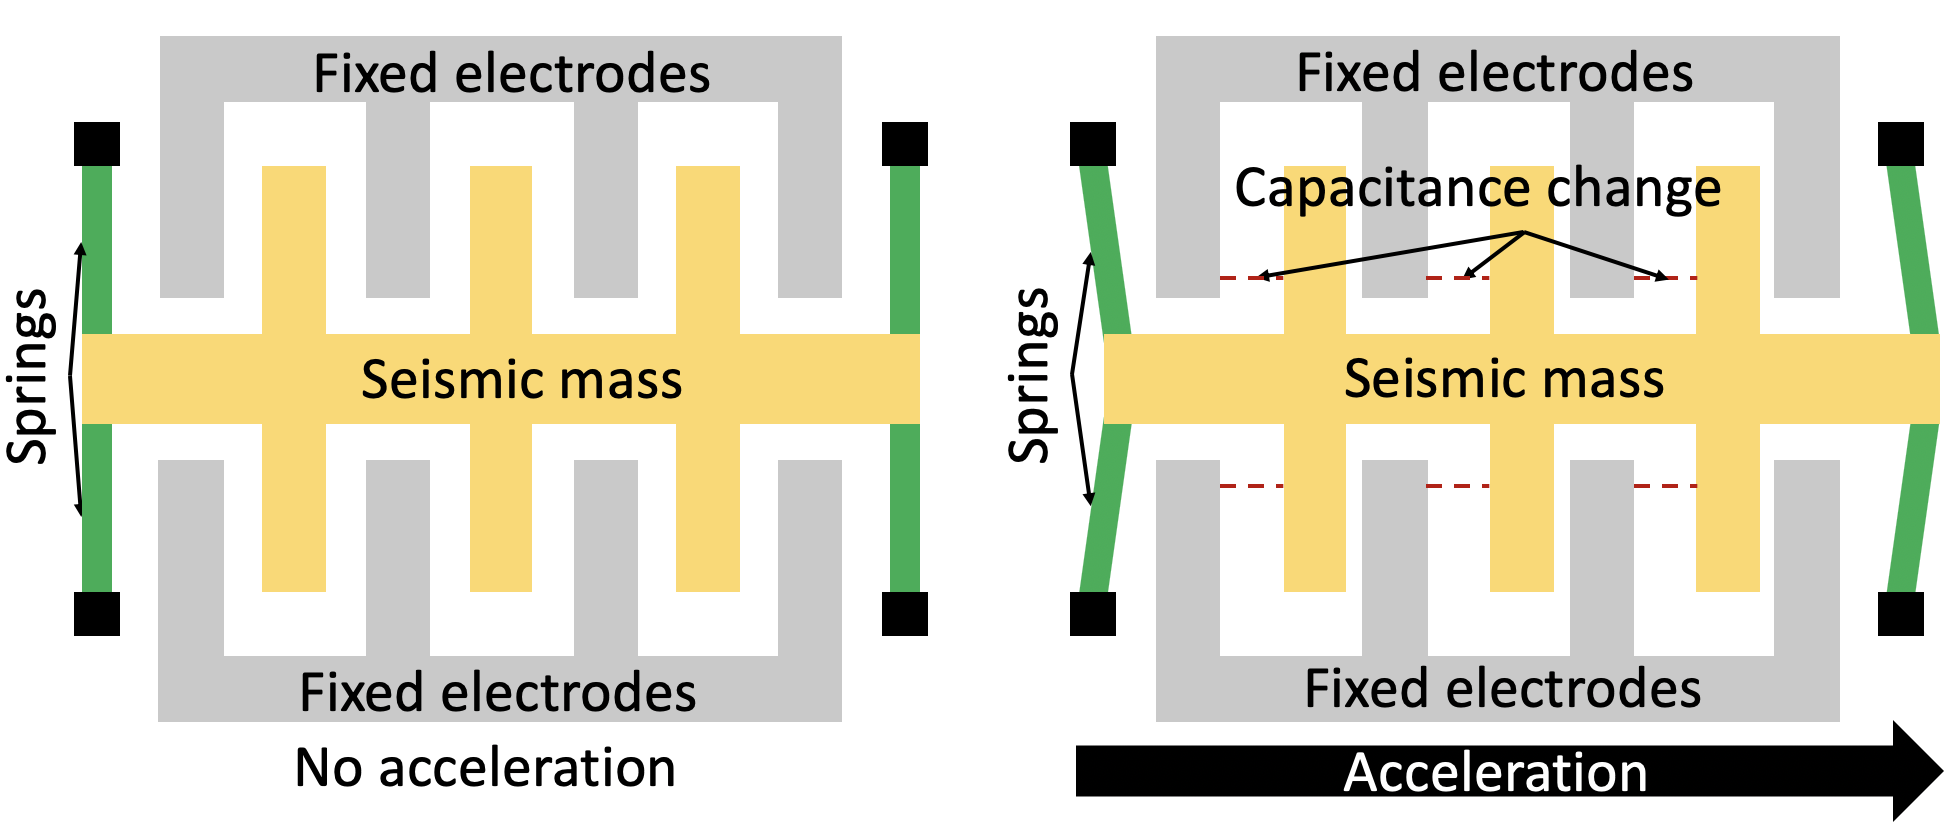
\includegraphics[width=\linewidth]{embed/MEMS_accelerometer.png}
  \caption{Accelerometer VC MEMS structure \cite{AccelEve2020}}
  \Description{Schematic of a MEMS accelerometer structure}
  \label{fig:MEMS_accelerometer}

  \vspace{0.25cm}

  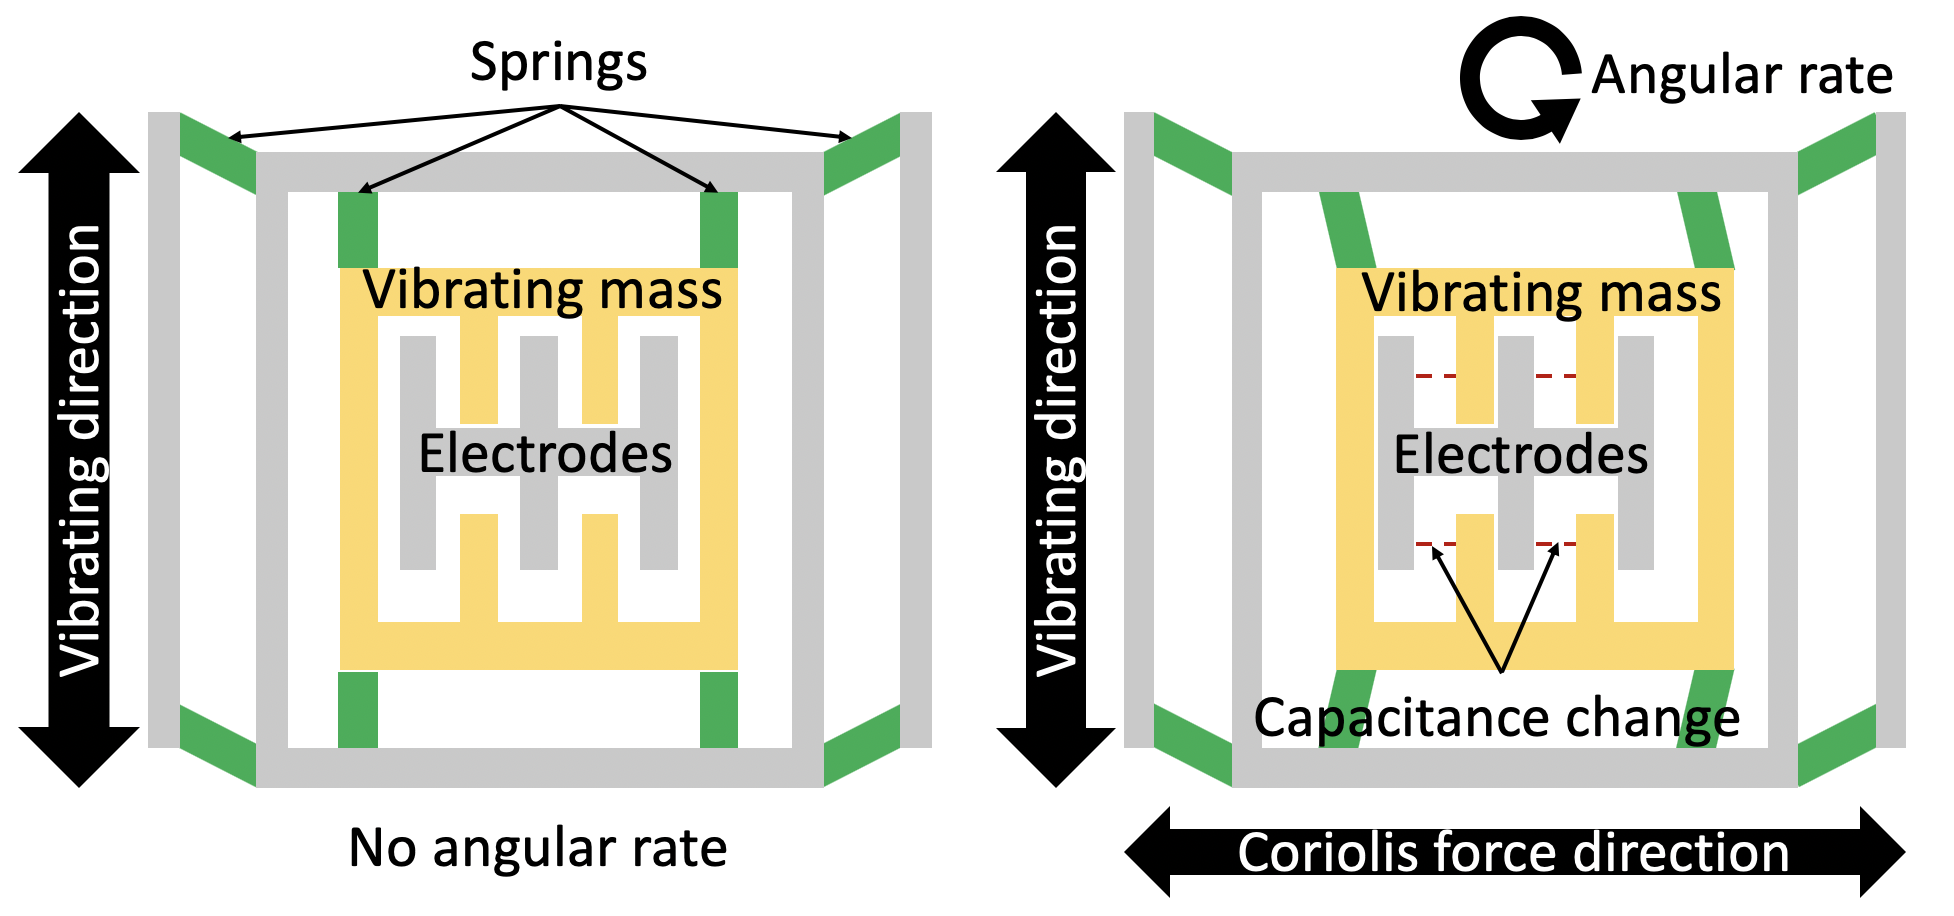
\includegraphics[width=\linewidth]{embed/MEMS_gyroscope.png}
  \caption{Gyroscope VC MEMS structure \cite{AccelEve2020}}
  \Description{Schematic of a MEMS gyroscope structure}
  \label{fig:MEMS_gyroscope}
\end{figure}

Although MEMS sensors are designed to be best insensitive to acoustic noise which could degrade their signal-to-noise ratio, they are still susceptible to sound waves that induce vibrations in the sensor structure.
A MEMS-based eavesdropping attack exploits this vulnerability by recovering the sound-induced vibrations from the sensor readings and reconstructing the original sound.
\\[6pt]
\textbf{Previous Work:} The first paper able to demonstrate the feasibility of recovering speech from motion sensors was \textit{Gyrophone: Recognizing Speech from Gyroscope Signals} \cite{Gyrophone2014} in 2014.
The authors showed that a smartphone's gyroscope can be used to recover speech rendered by a nearby loudspeaker using sensor readings at a well below Nyquist sampling rate of 200 Hz.
An Android app was developed to record the gyroscope readings without requiring any special permissions.
Later, they used the off-the-shelf Sphinx speech recognition system to recognize spoken digits, but also trained custom machine learning models to identify the speaker.

\subsection{Laser-based Eavesdropping Attacks}

\begin{figure}[h]
  \centering
  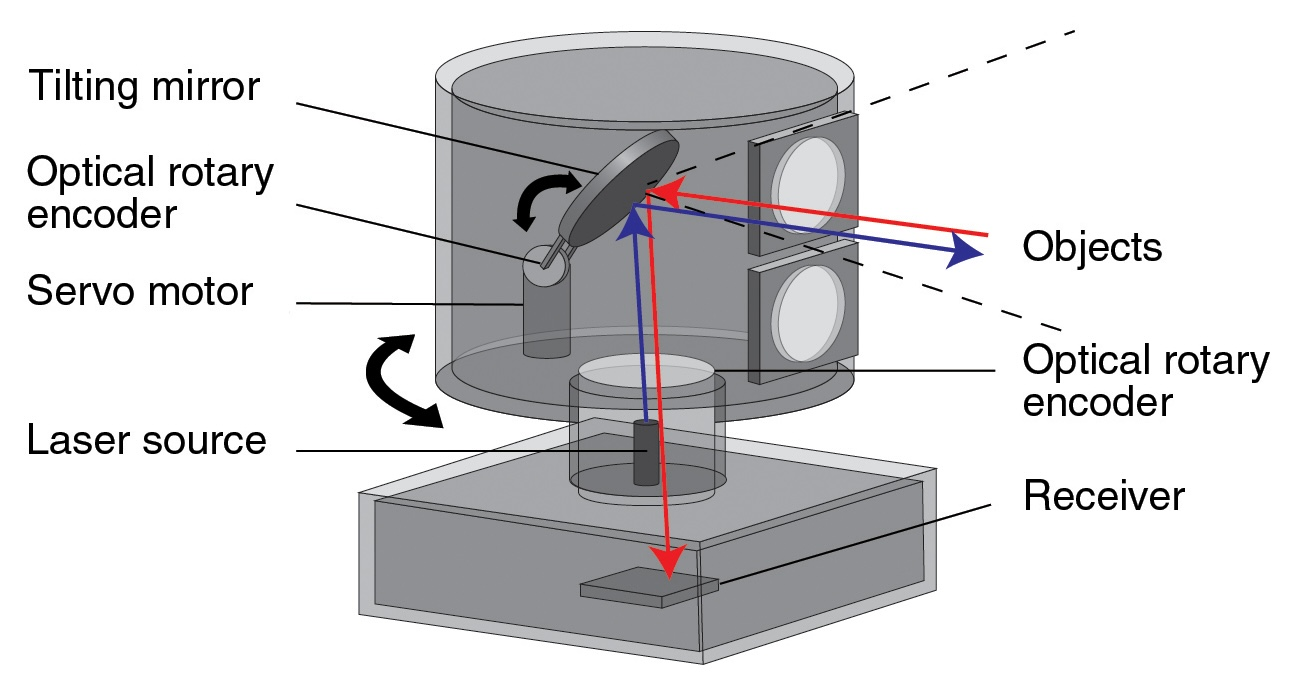
\includegraphics[width=\linewidth]{embed/Lidar_scanner.jpg}
  \caption{Mechanical spinning LiDAR \cite{RenishawLidar}}
  \Description{Schematic of a mechanical spinning LiDAR}

  \vspace{0.5cm}

  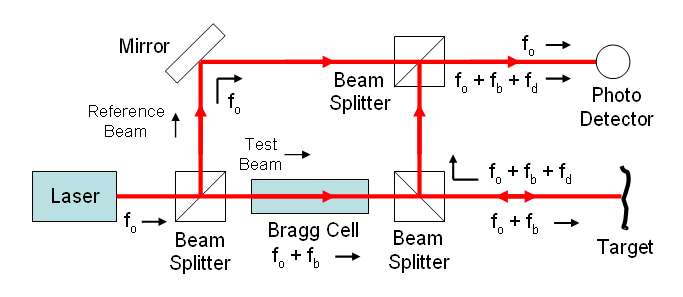
\includegraphics[width=\linewidth]{embed/Laser_Doppler_Vibrometer.png}
  \caption{Laser Doppler Vibrometer \cite{WikipediaLDV}}
  \Description{Schematic of a Laser Doppler Vibrometer}
\end{figure}

\subsection{Other Eavesdropping Attacks}
\section{Threat Model}
\section{Speech Reconstruction}
\subsection{Speech Intelligibility}
A human speeking in a non-tonal language like English produces a complex waveform that is composed of various frequencies in the audible range.
While the fundamental frequency $f_0$ of the human voice is typically in the range of 100 Hz to 300 Hz (higher for women and children), overtones and consonant articulations can cover most of the audible frequency range of up to 17 kHz (Figure \ref{fig:SpeechFrequencySpectrum}).
Research has shown that frequencies between 1 kHz and 4 kHz are most important for speech intelligibility \cite{DPAMicrophonesFactsAboutSpeechIntelligibility}.
Applying a low-pass filter to the speech signal at 1 kHz and below quickly degrades the intelligibility of the speech to near zero as shown in Figure \ref{fig:SpeechIntelligibility}.
Since most experimets conducted using motion sensors are limited to a sampling rate of 100-500 Hz, special techniques have to be employed to recover frequencies above the Nyquist frequency that are essential for speech intelligibility.

\begin{figure}[h]
  \centering
  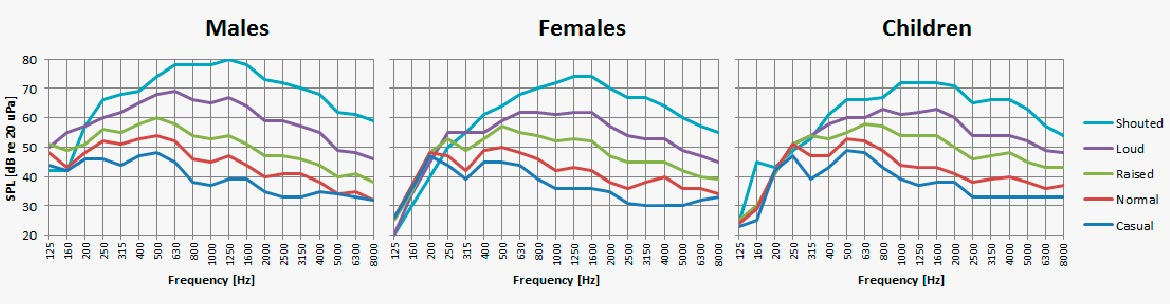
\includegraphics[width=\linewidth]{embed/Speech_frequency_spectrum.jpg}
  \caption{Frequency spectrum of a human voice for Males, Females and Children \cite{DPAMicrophonesFactsAboutSpeechIntelligibility}}
  \Description{Frequency spectrum of a human voice}
  \label{fig:SpeechFrequencySpectrum}

  \vspace{0.5cm}

  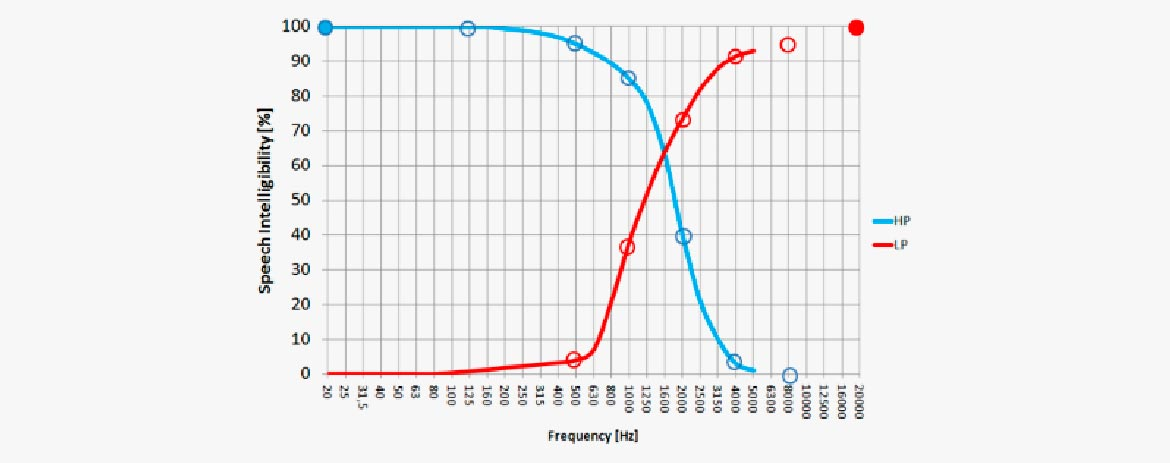
\includegraphics[width=\linewidth]{embed/Speech_Intelligibility_Low_High_Pass_Filter.jpg}
  \caption{Speech intelligibility with low-pass and high-pass filters applied at various frequencies \cite{DPAMicrophonesFactsAboutSpeechIntelligibility}}
  \Description{Speech intelligibility with low-pass and high-pass filters}
  \label{fig:SpeechIntelligibility}
\end{figure}

\subsection{Data Collection}
\subsection{Signal Processing}
\subsection{Machine Learning}
\subsection{Automated Speech Recognition}
\section{Feasibility Study}
\section{Countermeasures}
\section{Conclusion}

\begin{table*}[t]
  \caption{Test parameters and key results from previous publications on vibration-based speech recovery attacks exploiting different sensors}
\label{my-label}
\scriptsize
\renewcommand{\arraystretch}{1.3}
\begin{tabularx}{\textwidth}{@{} |lp{2.3cm}|*{7}{C}|r| @{}}
\toprule
\textbf{Year} & \textbf{Paper} & \textbf{Sensor} & \textbf{Attack Goal} & \textbf{Sampling Freq. (max)} & \textbf{Audio source} & \textbf{Transmission Medium} & \textbf{Distance from source} & \textbf{Dictionary Size} & \textbf{Accuracy (best)} \\
\hline
2014 & Gyrophone \cite{Gyrophone2014} & Gyroscope & Speech Recognition, Speaker Identification, Gender Identification & 200 Hz & External Loudspeaker & Solid Surface & 10 cm & 11 digits & 26 \% \\ \hline
2015 & AccelWorld \cite{AccelWorld2015} & Accelerometer & Speech Recognition, Speaker Identification & 200 Hz & External Loudspeaker & Air & 30 cm & 1 hotword & 85 \% \\ \hline
2017 & PitchIn \cite{PitchIn2017} & Accelerometer, Gyroscope, Geophone & Speech Recognition & 1 kHz & Human & Air & 1 m & 10 words & 79 \% \\ \hline
2018 & Speechless \cite{Speechless2018} & Accelerometer, Gyroscope & Speech Recognition & 8 kHz & External Loudspeaker & Solid Surface & 10 cm & 10 digits & 0 \% \\ \hline
2019 & Kinetic Song Comprehension \cite{KineticSongComprehension2019} & Accelerometer, Gyroscope & Song Recognition & 100 Hz & Smartphone Loudspeaker & Solid Surface & On-Device & 100 songs & 80 \% \\ \hline
2020 & AccelEve \cite{AccelEve2020} & Accelerometer & Speech Recognition, Speaker Identification & 500 Hz & Smartphone Loudspeaker & Solid Surface & On-Device & 8 hotwords & 90 \% \\ \hline
2021 & Spearphone \cite{Spearphone2021} & Accelerometer & Speech Recognition, Speaker Identification, Gender Identification & 500 Hz & Smartphone Loudspeaker & Solid Surface & On-Device & 58 words & 67 \% \\ \hline
2021 & Vibphone \cite{Vibphone2021} & Accelerometer & Speech Recognition & 170 Hz & Smartphone Loudspeaker & Solid Surface & On-Device & 10 hotwords + 10 digits & 54.2 \% \\ \hline
2022 & AccMyrinx \cite{AccMyrinx2022} & Accelerometer & Speech Recognition & 500 Hz & Smartphone Loudspeaker & Solid Surface & On-Device & Synthesis & 57.33 \% \\ \hline
2023 & ISpyU \cite{ISpyU2023} & Accelerometer, Gyroscope & Continuous Speech Recognition & 500 Hz & Smartphone Loudspeaker & Solid Surface & On-Device & 9950 words & 53.3 \% \\ \hline
2023 & VoiceListener \cite{VoiceListener2023} & Accelerometer, Gyroscope, Magnetometer & Speech Recognition & 250 Hz & Smartphone Loudspeaker & Solid Surface & On-Device & 10 digits & 82.7 \% \\ \hline
2024 & Watch the Rhythm \cite{WatchTheRhythm2024} & Accelerometer & Speech Recognition & 200 Hz & Smartphone Loudspeaker & Solid Surface & On-Device & 10 digits & 77.79 \% \\
\hline\hline
2020 & Lidarphone \cite{Lidarphone2020} & Lidar Scanner & Speech Recognition, Speaker Identification, Gender Identification & 1.8 kHz & External Loudspeaker & Air & 1.5 m & 10 digits & 91 \% \\
\hline\hline
2019 & Hard Drive of Hearing \cite{HardDriveOfHearing2019} & Hard Drive PES & Speech Recognition & 34.56 kHz & External Loudspeaker & Air & 25 cm & - & - \\
\bottomrule
\end{tabularx}
\end{table*}

%%
%% The acknowledgments section is defined using the "acks" environment
%% (and NOT an unnumbered section). This ensures the proper
%% identification of the section in the article metadata, and the
%% consistent spelling of the heading.
% \begin{acks}
% To Robert, for the bagels and explaining CMYK and color spaces.
% \end{acks}

%%
%% The next two lines define the bibliography style to be used, and
%% the bibliography file.
\newpage
\bibliographystyle{ACM-Reference-Format}
\bibliography{references}


%%
%% If your work has an appendix, this is the place to put it.
% \appendix

\end{document}
\endinput
%%
%% End of file `sample-sigconf.tex'.
